\usetikzlibrary{arrows.meta}
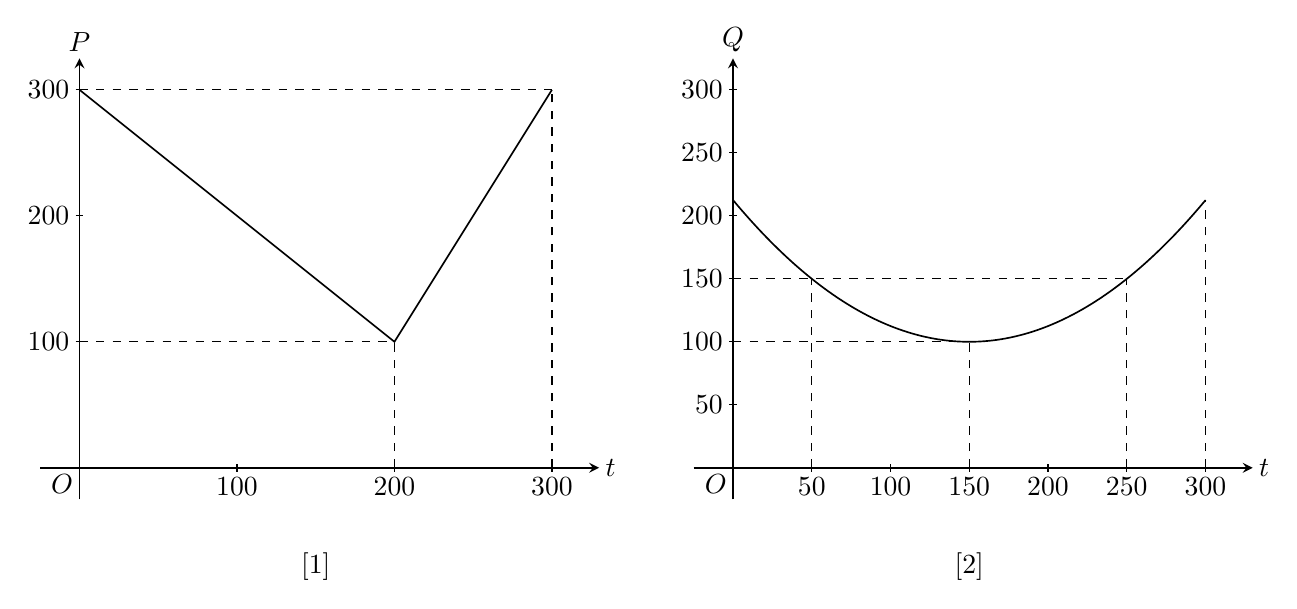
\begin{tikzpicture}[x=1cm,y=1cm,line width=.6pt,>=stealth,font=\normalsize]
\draw[->] (-0.5,0)--(6.6,0) node[right,inner sep=0pt,xshift=2pt] {$t$};
\draw[->] (0,-0.4)--(0,5.2) node[above,inner sep=0pt,yshift=2pt] {$P$};
\node[anchor=north east,inner sep=0pt,xshift=-2pt,yshift=-2pt] at (0,0) {$O$};
\draw[line width=.45pt] (2.00,-0.05)--(2.00,0.05);
\node[anchor=north,inner sep=0pt,yshift=-2pt] at (2.00,-0.05) {$100$};
\draw[line width=.45pt] (4.00,-0.05)--(4.00,0.05);
\node[anchor=north,inner sep=0pt,yshift=-2pt] at (4.00,-0.05) {$200$};
\draw[line width=.45pt] (6.00,-0.05)--(6.00,0.05);
\node[anchor=north,inner sep=0pt,yshift=-2pt] at (6.00,-0.05) {$300$};
\draw[line width=.45pt] (-0.05,1.60)--(0.05,1.60);
\node[anchor=east,inner sep=0pt,xshift=-2pt] at (-0.05,1.60) {$100$};
\draw[line width=.45pt] (-0.05,3.20)--(0.05,3.20);
\node[anchor=east,inner sep=0pt,xshift=-2pt] at (-0.05,3.20) {$200$};
\draw[line width=.45pt] (-0.05,4.80)--(0.05,4.80);
\node[anchor=east,inner sep=0pt,xshift=-2pt] at (-0.05,4.80) {$300$};
\draw[dashed,line width=.45pt] (0,4.8)--(6.0,4.8) (0,1.6)--(4.0,1.6) (4.0,0)--(4.0,1.6) (6.0,0)--(6.0,4.8);
\draw (0,4.8)--(4.0,1.6)--(6.0,4.8);
\node[anchor=north,inner sep=0pt,yshift=-2pt] at (3.0,-1.0) {\bitmapinsertcaption[1]};
\begin{scope}[xshift=8.3cm]
\draw[->] (-0.5,0)--(6.6,0) node[right,inner sep=0pt,xshift=2pt] {$t$};
\draw[->] (0,-0.4)--(0,5.2) node[above,inner sep=0pt,yshift=2pt] {$Q$};
\node[anchor=north east,inner sep=0pt,xshift=-2pt,yshift=-2pt] at (0,0) {$O$};
\draw[line width=.45pt] (1.00,-0.05)--(1.00,0.05);
\node[anchor=north,inner sep=0pt,yshift=-2pt] at (1.00,-0.05) {$50$};
\draw[line width=.45pt] (2.00,-0.05)--(2.00,0.05);
\node[anchor=north,inner sep=0pt,yshift=-2pt] at (2.00,-0.05) {$100$};
\draw[line width=.45pt] (3.00,-0.05)--(3.00,0.05);
\node[anchor=north,inner sep=0pt,yshift=-2pt] at (3.00,-0.05) {$150$};
\draw[line width=.45pt] (4.00,-0.05)--(4.00,0.05);
\node[anchor=north,inner sep=0pt,yshift=-2pt] at (4.00,-0.05) {$200$};
\draw[line width=.45pt] (5.00,-0.05)--(5.00,0.05);
\node[anchor=north,inner sep=0pt,yshift=-2pt] at (5.00,-0.05) {$250$};
\draw[line width=.45pt] (6.00,-0.05)--(6.00,0.05);
\node[anchor=north,inner sep=0pt,yshift=-2pt] at (6.00,-0.05) {$300$};
\draw[line width=.45pt] (-0.05,0.80)--(0.05,0.80);
\node[anchor=east,inner sep=0pt,xshift=-2pt] at (-0.05,0.80) {$50$};
\draw[line width=.45pt] (-0.05,1.60)--(0.05,1.60);
\node[anchor=east,inner sep=0pt,xshift=-2pt] at (-0.05,1.60) {$100$};
\draw[line width=.45pt] (-0.05,2.40)--(0.05,2.40);
\node[anchor=east,inner sep=0pt,xshift=-2pt] at (-0.05,2.40) {$150$};
\draw[line width=.45pt] (-0.05,3.20)--(0.05,3.20);
\node[anchor=east,inner sep=0pt,xshift=-2pt] at (-0.05,3.20) {$200$};
\draw[line width=.45pt] (-0.05,4.00)--(0.05,4.00);
\node[anchor=east,inner sep=0pt,xshift=-2pt] at (-0.05,4.00) {$250$};
\draw[line width=.45pt] (-0.05,4.80)--(0.05,4.80);
\node[anchor=east,inner sep=0pt,xshift=-2pt] at (-0.05,4.80) {$300$};
\draw[dashed,line width=.45pt] (0,2.4)--(5.0,2.4) (0,1.6)--(3.0,1.6) (1.0,0)--(1.0,2.4) (3.0,0)--(3.0,1.6) (5.0,0)--(5.0,2.4) (6.0,0)--(6.0,3.4);
\draw[domain=0:300,samples=121] plot ({0.02*\x},{1.6+(\x-150)/100*(\x-150)/100*0.8});
\node[anchor=north,inner sep=0pt,yshift=-2pt] at (3.0,-1.0) {\bitmapinsertcaption[2]};
\end{scope}
\end{tikzpicture}
